%!TeX root = Chapter_ComputationalMethods
\documentclass[../../CompleteThesis/Complete_1stDraft.tex]{subfiles}

\begin{document}
	
	\section[Splines and Interpolation]{Splines and Interpolation}	
	\label{Sec:CompMeths_SplinesAndInterpolation}
	\subsection[Interpolation][Interpolation]{Interpolation}
	\label{Subsec:CompMeths_SplinesAndInterpolation_Interpolation}
	Interpolation is a tool that can be used - and misused - to extract more information out of a given set of data. Used correctly, interpolation can reveal more information than is initially available and disclose connections not apparent at first, but used incorrectly, it can be manipulated to infer misleading correlations and lead to inaccurate conclusions. Thus it is a tool that must be used with care. Aiming to avoid incorrect deductions and inferences one should at first gain as much knowledge about the data at hand as possible. By understanding how the data have come about and gaining knowledge about the underlying physical theories a somewhat deficient data set can robustly and securely be interpolated to accommodate the needs of the analysis. In the case of this thesis, both knowledge about data gathering and the physics at play have been gained and thus some of the common fallacies may be avoided. The limits of the data available is due to the discrete sampling, leading to a minimum sampling of about 26 samples per meter of ice.
	When considering that the depth series of 32 years between Tambora and Laki is just above 10 meters, this means that each meter of ice needs to contain at least three years on average. 26 samples per three years might not sound as a bad sampling interval, but if the goal is to show seasonality and give a best estimate of annual layer thickness, interpolation could be put to good use to be able to give better estimates of the exact placement of peaks and valleys.\\	\subsubsection[Basic Idea][Basic Idea]{Basic Idea}
	\label{Subsubsec:CompMeths_SplinesAndInterpolation_Interpolation_BasicIdea}
	\todo{Write short introduction to interpolation here. Reference Appendix.}
	
	\subsection[Interpolation in this Project][Interpolation in this Project]{Cubic Spline Interpolation in this Project}
	\label{Subsec:CompMeths_SplinesAndInterpolation_InterpolationInThisProj}
	For this project cubic spline interpolation has been implemented and examined in two particular sections of the analysis: 
	\begin{enumerate}
		\item Cubic spline interpolation of raw, uneven data to represent even data, that can be analyzed through fast spectral transforms.
		\item Cubic spline interpolation of the final back-diffused signal estimate to enhance resolution for more efficient peak detection.
	\end{enumerate}
	
	\subsubsection[Interpolation 1]{Interpolation of Data Before Deconvolution}
	\label{Subsubsec:CompMethod_StabilityTests_Interpolation1}
	
	The first interpolation is needed, if the fast spectral transforms FFT or FCT are used, as one of the conditions of the algorithms is that the data are evenly spaced. At first, this was implemented in the analysis, but this had the risk of excluding some information that might lie in the unevenly sampled data. Later, the method was abandoned in favor of implementing a nonuniform spectral transform (NUFT or NDCT), which is slower than the FFT and FCT, but carries all information from the unevenly sampled signal into the spectral domain. Luckily, this nonuniform transform needs only be carried out once, as the inverse transform, i.e. resampling in time domain, can be done uniformly without loss of information and any future spectral transforms can then be performed through FFT or FCT.
	Even though the first interpolation method was later abandoned, some analysis was carried out with it to examine the effect of the size of the resampled, interpolated data on the final diffusion length estimate. Examples of a resampled signal can be seen in Figure \ref{Fig:COMPMETH_SiteA_DataSplineInterp} and Figure \ref{Fig:COMPMETH_SiteA_MultiSplineInterp}. Figure \ref{Fig:COMPMETH_SiteA_MultiSplineInterp} shows how sample resolution affects information from the signal. The higher sampling resolution, the more information is retained. But higher sampling resolution also means more data to be analyzed, which might slow down any analysis algorithms developed. This might create some headache if an entire ice core length of a couple thousand meters should be examined, but for this study only af few meters are of interest, and thus it should not create delays in the computation time.
	
	\begin{figure}[h]
		\centering
		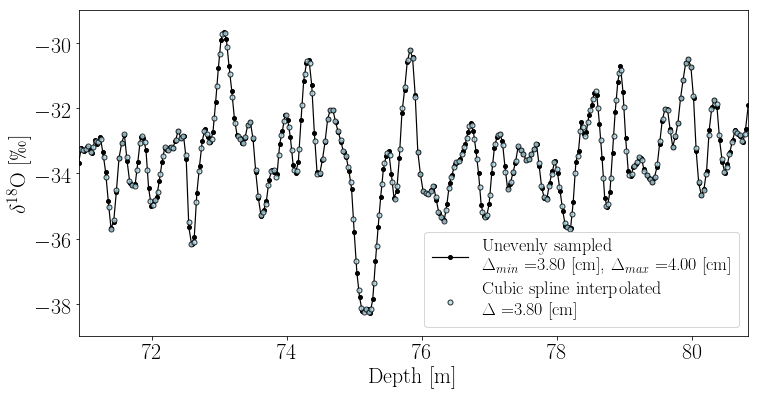
\includegraphics[width=\textwidth]{SiteA_DataSplineInterp.png}
		\caption{Unevenly sampled signal from Site A resampled using cubic spline interpolation to an even signal with a new sample size equal to the minimum sample size found in the raw signal.}
		\label{Fig:COMPMETH_SiteA_DataSplineInterp}
	\end{figure}
	
	\begin{figure}[h]
		\centering
		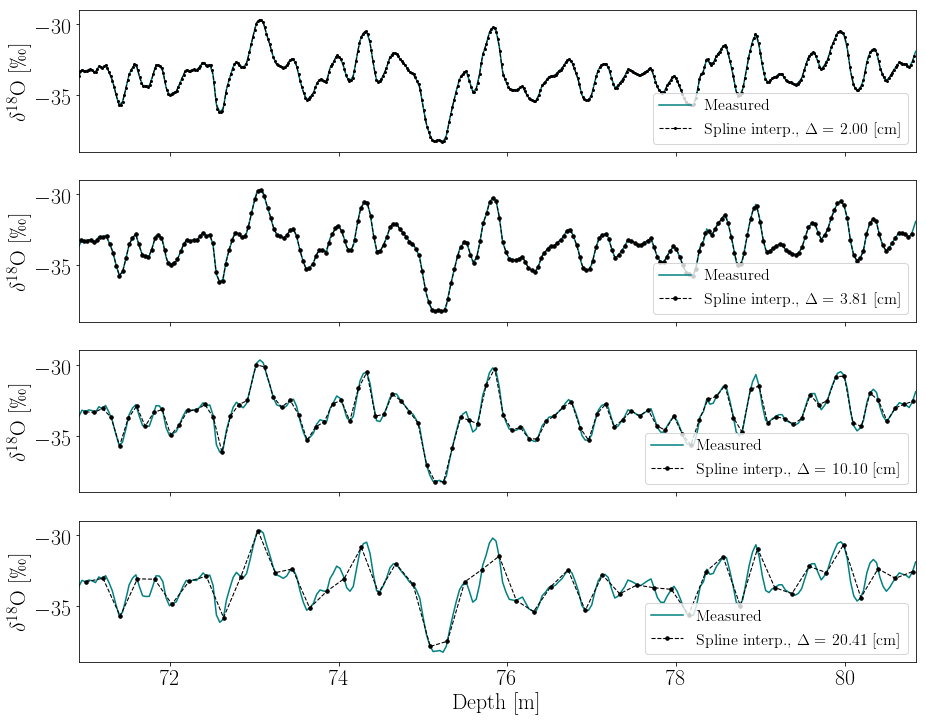
\includegraphics[width=\textwidth]{SiteA_MultiSplineInterp.png}
		\caption{Four different resampled signals of Site A data, showing loss of information when resampling resolution is low.}
		\label{Fig:COMPMETH_SiteA_MultiSplineInterp}
	\end{figure}
	
	To examine the effect of the resampling resolution on the final diffusion length estimate when conducting a spline interpolation before carrying out the back-diffusion, the full diffusion length analysis has been performed with 100 new interpolation resampling sizes in the range $[\Delta_{\text{min}};\Delta_{\text{max}}]$. This gives an idea of the stability of the method considering both sample size of the raw data and resampling by interpolation. The minimum and maximum interpolation samplings are presented in Table \ref{tab:InterpSamples} and an illustration of the test results can be seen in Figure \ref{Fig:COMPMETH_SamplingVsDiffLen_interpBF}.
	
	\marginnote{%
		\footnotesize
		\centering
		\begin{tabular}{lcc}
			\toprule
			\textbf{Site} & $\Delta_{\text{min}}$& $\Delta_{\text{max}}$\\
			& [m] & [m] \\
			\midrule
			Crete & 0.02 & 0.13 \\
			Site A & 0.022 & 0.12 \\
			Site B & 0.01 & 0.14 \\
			Site D & & \\
			Site E & 0.02 & 0.12 \\
			Site G & 0.02 & 0.11 \\
			\bottomrule
		\end{tabular}
		\captionof{table}{\footnotesize Minimal and maximal new sample resolution used for testing interpolation before back-diffusion. Each test is run with 100 different new sample resolutions between $\Delta_{\text{min}}$ and $\Delta_{\text{max}}$.}
		\label{tab:InterpSamples}
	}[0.5cm]%
	
	
	\begin{figure}[h]
		\centering
		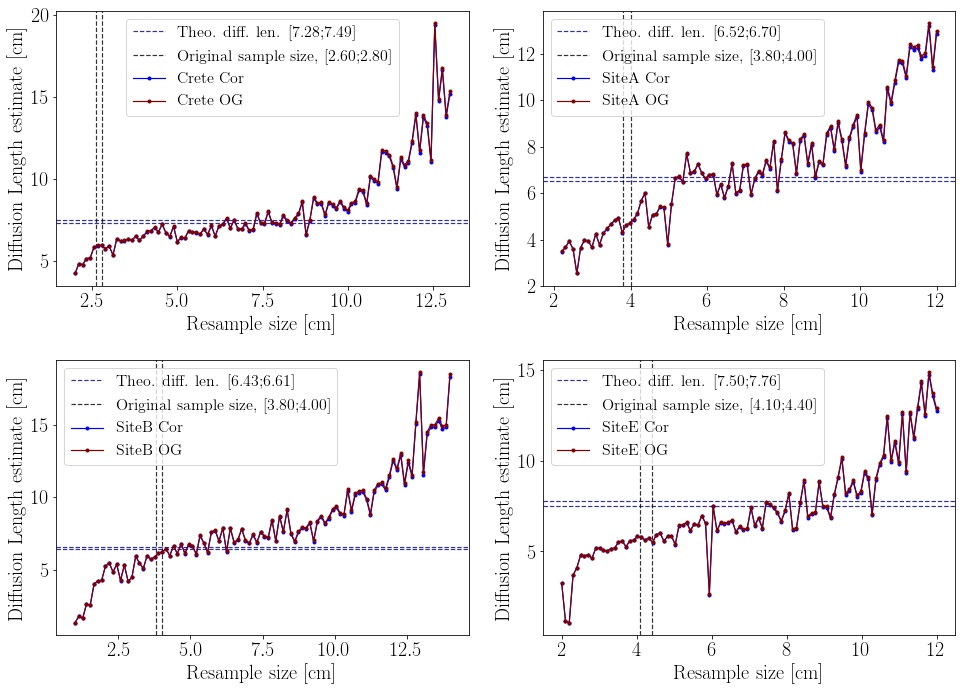
\includegraphics[width=\textwidth]{SamplingVsDiffLen_interpBF.jpg}
		\caption{}
		\label{Fig:COMPMETH_SamplingVsDiffLen_interpBF}
	\end{figure}
	
	\todo{COMPMETH: Write figure captions to all figures.}
	
	
	\subsubsection[Interpolation 2]{Interpolation of Data After Deconvolution}
	\label{Subsubsec:CompMethod_StabilityTests_Interpolation2}
	The second interpolation is carried out after deconvoluting and back-diffusing the signal, but before detecting peaks. Splines are especially effective when trying to find features like peaks in data which underlying signal is continuous, smooth and differentiable, but the sampling is discrete and thus the data are discrete and non-smooth. The isotopic signal under examination here is assumed to be truly smooth and continuous throughout the core - unless any gaps are present. Thus the cubic spline interpolation is a good tool for estimating a higher resolution version of the final back-diffused data series to use for peak detection. This makes the detection of peaks and troughs more precise, as there might not be a discrete data point exactly at the top of a peak, but the spline interpolation then estimates where the most likely top of the peak must be, on the basis of the existing data. Examples of three different interpolation samplings are presented in Figure \ref{Fig:COMPMETH_SiteA_InterpAF_4samplings}. The effect of resampling after deconvolution on the final diffusion length estimate is illustrated in Figure \ref{Fig:COMPMETH_SamlingVsDiffLen}.
	
	\begin{figure}[h]
		\centering
		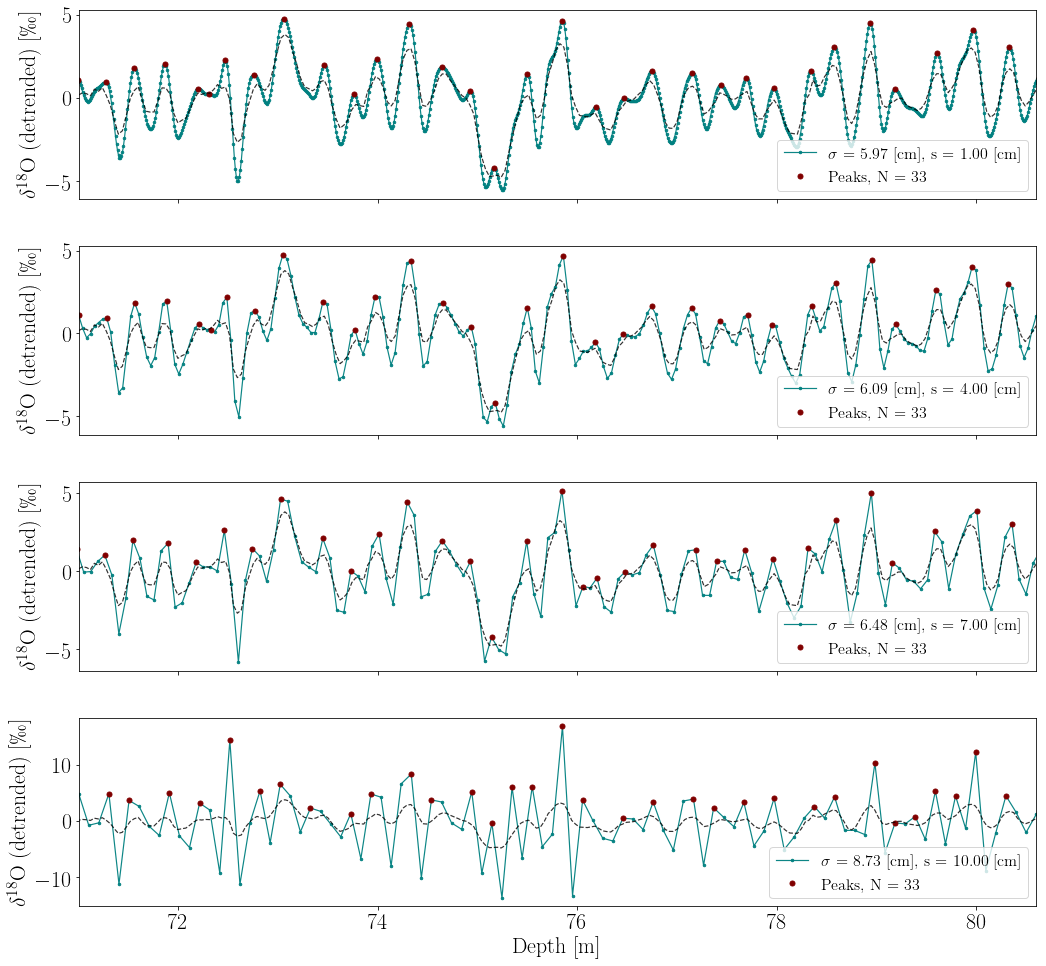
\includegraphics[width=\textwidth]{SiteA_InterpAF_4samplings.png}
		\caption{}
		\label{Fig:COMPMETH_SiteA_InterpAF_4samplings}
	\end{figure}
	
	\begin{figure}[h]
		\centering
		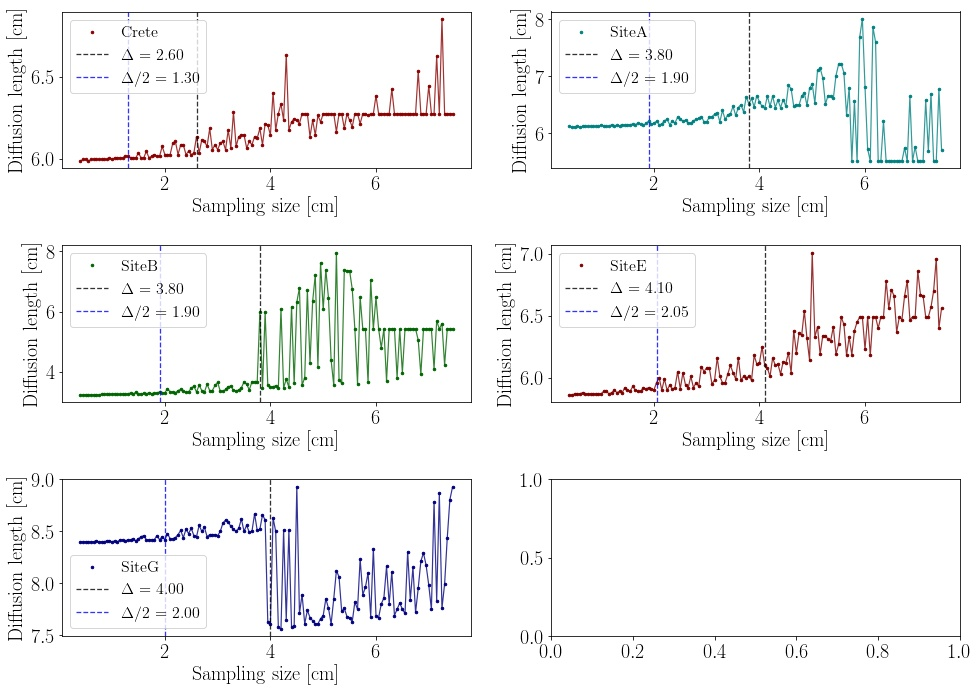
\includegraphics[width=\textwidth]{SamlingVsDiffLen.jpg}
		\caption{}
		\label{Fig:COMPMETH_SamlingVsDiffLen}
	\end{figure}
	
	\section[Peak Detection]{Peak Detection}
	\label{Sec:CompMeths_PeakDetection}
	
	Knowing that water isotopic data are a proxy for temperature, the most obvious way to determine annual layers in the signals is by detecting peaks and troughs. During colder periods, e.g. winter, the air masses arriving at the ice core sites have formed more precipitation before reaching the sites, and the vapor that results in this final precipitation is then more depleted of heavy isotopes, resulting in lower isotopic values, troughs in Figure \ref{Fig:ICE_Crete_10m_dated}. The precipitation falling during warmer conditions, e.g. summer, is correspondingly less depleted of the heavy isotopes, and results in higher isotopic values, peaks in Figure \ref{Fig:COMPMETH_Crete_10m_PeaksTroughs}.
	\begin{figure}[h]
		\centering
		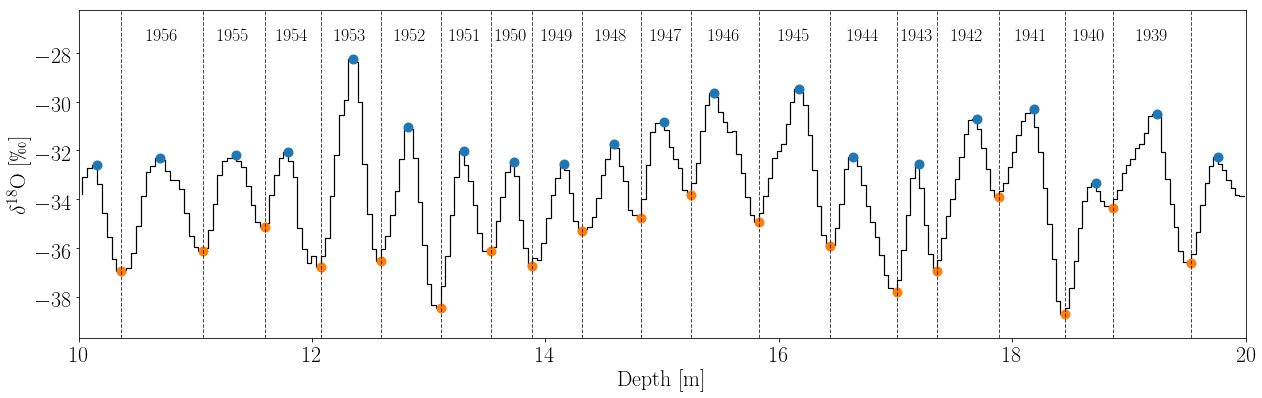
\includegraphics[width=\textwidth]{Crete_10m_PeaksTroughs.png}
		\caption{Ten meters of the top of Cretê ice core, with identification and dating of 19 annual layers, with peaks(blue) corresponding to summers and troughs(orange) corresponding to winters.}
		\label{Fig:COMPMETH_Crete_10m_PeaksTroughs}
	\end{figure}
	Peak detection and layer counting has previously been carried out by visual inspection of the ice core depth signals, but as computers and algorithms have become more integrated in data analysis, it is now more common to use different computational methods. Developing and implementing layer counting and peak detection algorithms can be done in a number of different ways, but for this project, at first a very simple method has been initially implemented and later the method has been improved and optimized through a number of different constraints. One could also use different pattern recognition techniques[REFERENCE]\todo{References here.} to achieve more intelligent detection, and later some of these methods will be presented.\\
	The most naïve approach, and the one first implemented in this project, to peak detection is to simply find local maxima by comparing neighbouring values. When examining point $d_i$, the point is deemed a local maxima, if $d_{i\pm1} < d_i$. Local minima, troughs, can be found in exactly the same manner by finding minima as $d_{i\pm1} > d_i$. A very simple constraint for this method is to keep a required minimal distance between peaks, so that two peaks cannot be detected within a point distance of $\Delta d_{\text{min}}$. For example at a depth of 12 m in Figure \ref{Fig:COMPMETH_Crete_10m_PeaksTroughs} two troughs can be seen, but only one is chosen, as they are within the threshold distance to each other, which here is set to $\Delta d_{\text{min}} = 7$ points. Here, the lowest of the two troughs is chosen. The threshold distance can be chosen in different ways, for this short section it has been chosen through visual inspection, but more generally it can be chosen by examining some of the intrinsic properties of the signal, more about this in Section \ref{}.
	
	\todo{COMPMETH-PEAKDET: Write about better peak detection with cubic spline interpolation (enhanced resolution)}
	
	

	
\end{document}
